
\begin{question}
Consider LakeHuron time series.

You can load the LakeHuron data set in R by issuing the following command at the console data(``LakeHuron'') or if you use other programming languages you can download it \href{https://github.com/vincentarelbundock/Rdatasets/blob/master/csv/datasets/LakeHuron.csv}{here}.

\begin{figure}[H]
\centering
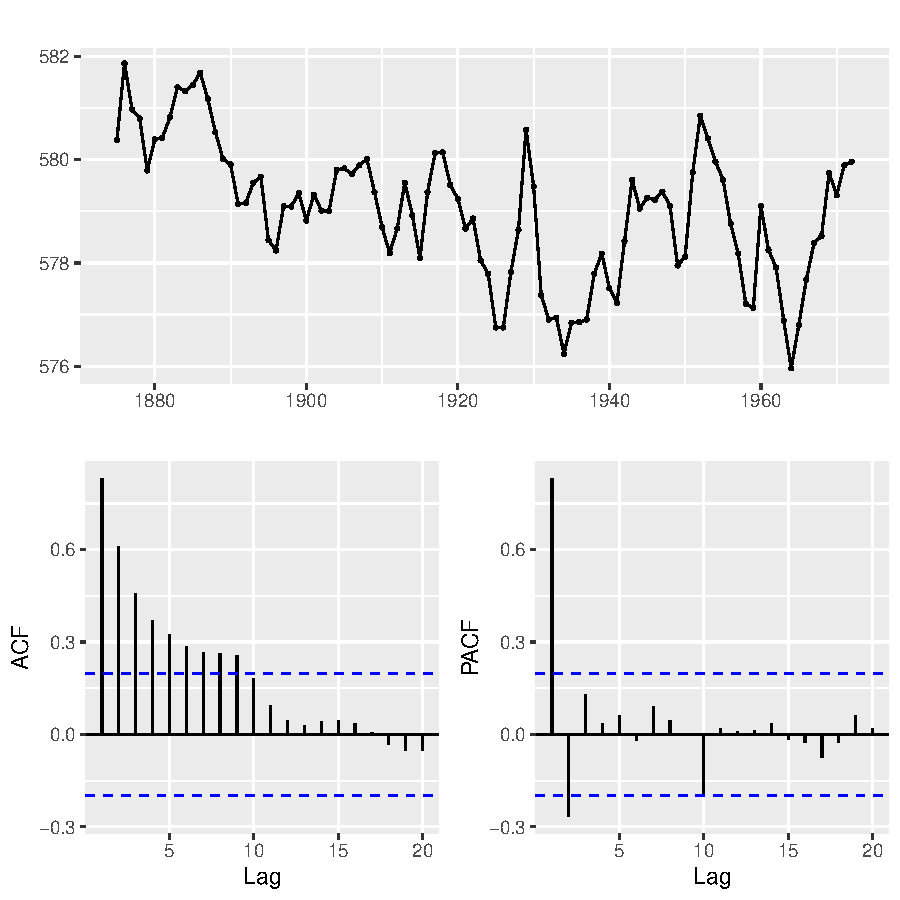
\includegraphics{unnamed-chunk-1-1-3.pdf}
\caption{plot of chunk unnamed-chunk-1}
\end{figure}

By analysing ACF and PACF functions answer, what can the underlying ARMA(p,q) process be?
\begin{answerlist}
  \item ARMA(0,1)
  \item ARMA(1,0)
  \item ARMA(1,1)
  \item ARMA(2,0)
  \item ARMA(0,0)
  \item ARMA(0,2)
\end{answerlist}
\end{question}

\begin{solution}
A gradual geometrically declining ACF and with PACF that is significant for only 2 lags indicate an AR process. Since the number of observations is not large enough the significance of PACF(2) is questionable.
\end{solution}

